\section{Implementation}

\subsection{Methodology}

Due to the many initial unknowns and research-driven approach influencing the system design, an Agile mind-set was taken from the start to support changing requirements and iterative working releases.

This proved really useful as many decisions have had to be made after the implementation began and a few compromises have happened, which can be seen from the system design section.

Requirement gathering and the development of testing scenarios also took an Agile approach. Due to the technical aspect of the app, it was easier for users to drive the development after they were able to use the initial version on their own. This has meant that many requirements were obtained after the first iteration finished.

As presented in the System design section, a number of user stories were thought of mainly from the perspective of the Dashboard and were used to drive the development of the entire system. 

\subsection{JNI/JVMTI Agent Library}
For the purpose of gaining performance, not many unneeded libraries have been used. A small logging library has been built from scratch and handles only console output if enabled.

After the heap is reconstructed in the internal data-structure, an XML is built and sent to a thread pending delivery to the API engine.

Handlers have been coded to process the different kinds of primitives and objects that programmers can create in the JVM. Many different edge cases have stood out during research and testing, such as the difference between static and instance fields.

\subsubsection{Requirements on the JVM app owner side}
To deliver any of its promises, the agent requires the Java app to be built using either the defaults for the javac -g option or javac -g:lines,vars. This lets the compiler know that it should also record useful debugging information in the .class files, such as the local variable names \cite{javac}.

Local variables names and line numbers are recorded by default if no -g is specified.

\subsubsection{Mapping primitive, array and object types}

A hashmap data structure based around the object id is created on the native agent side as a mid-transition-point between the JVM heap and the construction of the message sent to the API.

The unique (per exception) object id used to identify an object is obtained using the JVMTI.GetObjectHashCode method which guarantees the returned integer hashcode is different for all objects across their lifetime \cite{GetObjectHashCode}. 

Every single variable is represented in the following data-structure on the agent side regardless of its properties:

\begin{listing}[H]
\begin{minted}[breaklines=true]{c}
struct VarHolder {
  int object_id;
  char * name;
  char * signature;
  char * generic;

  char * value;
  int array_length;
  bool is_static;

  int field_count;
  VarHolder * fields;
}
\end{minted}
\caption{Variable wrapper on the Agent side}
\end{listing}

The code is show so that the reader can build a mental-model of how the system works behind the scenes.

The fields list represents in the case of
\begin{itemize}
  \item an array, each entry held within
  \item an object, each static and non-static field
\end{itemize}

To reduce the complexity of the code needed to handle the processing of variable types, the value/contents of objects (non-primitive variables), where they are not null, is currently established by calling the .toString method using the JNI.CallObjectMethod \cite{jniMethod}. Primitives can be parsed from string into their original format via later processing based on their recorded type.

~\\

The following table defines the mapping used \cite{jniTypes}.

\begin{listing}[H]

\begin{center}
    \begin{tabular}{ |l|l| }
      \hline
        Type Signature & Java Type \\
      \hline
      Z & boolean \\
            \hline

      B & byte \\
            \hline

      C & char \\
            \hline

      S & short \\
            \hline

      I & int \\
            \hline

      J & long \\
            \hline

      F & float \\
            \hline

      D & double \\
            \hline

      L fully-qualified-class & Object / Custom class \\
            \hline

      {[} type & Array of type \\
      \hline

    \end{tabular}
\end{center}

\caption{Mapping type signature to java types}
\end{listing}

All the types before L are considered to be a primitive type. 

\subsubsection{Parsing variable contents recursively}

The following pseudo-code explains on a very high-level how the agent obtains the values it needs to represent the state of each frame/method/stack-entry of a stack-trace:

\begin{listing}[H]
\begin{minted}[breaklines=true]{c}
function to processVariable given var
    if var is a primitive
        handle value according to type 
    if var is an array
        for each entry in var.elements
            processVariable (entry)
    if var is an object
        for each field in var.fields
            processVariable (field)

function to processStackTrace given stack-trace           
    for each frame in stack-trace
        stackLocalVars <- local variables of current frame
        for each var in stackLocalVars
            processVariable (var)
        staticVariables <- static variables of current frame object used in the frame
        for each var in staticVariables
            processVariable (var)
\end{minted}
\caption{High-level pseudo-code for obtaining values of variables on a stack-trace}
\end{listing}

The actual code under the processVariable function changes depending on whether the variable is static or local.

There are a few cases to consider when dealing with variables
\begin{itemize}
  \item Are they locally defined?
  \item Are they static variables? 
  \item Are they arrays?
  \item Are they objects?
\end{itemize}

If we are dealing with objects then the agent will explore all the fields defined for them. The JVMTI provides a method named GetClassFields which is used for that purpose. Each field is then handled in the same way recursively, for example are any of the fields a primitive, an object or an array?

The same pattern is used for handling arrays, only that the fields are considered to be the entries in the array.

GetClassFields will return both static and instance fields of a class of an object. To extract values from each of these fields, a different call to JNI must be used depending on if they are statically or instance/locally defined. For example, JNI.GetStaticIntField / JNI.GetIntField  \cite{jnibook}. 

\subsubsection{Native callback when an exception is detected}

\begin{listing}[H]
\begin{minted}[breaklines=true]{c}
void JNICALL callbackException(jvmtiEnv *jvmti_env, JNIEnv* env, jthread thr, jmethodID method, jlocation location, jobject exception, jmethodID catch_method, jlocation catch_location)
\end{minted}
\caption{JVMTI Exception callback to native agent}
\end{listing}


This is one of the very first parts the native agent implemented, which is to listen to the callback from the JVMTI event jvmtiEventException with pointers to the exception. 

The JVM waits until this call is completed so the processing of the stack-trace needs to be quick and the API communication has to be handled in a different thread so as to slow down the JVM as less as possible.

\subsubsection{Edge case: native exceptions}
During experimentation it has been revealed that on start-up the JVM throws a few exceptions, mainly due to class loaders, and handles them by itself.

The agent picked up these exceptions which this reports refers to as native exceptions, and they are hard-coded as white-labelled in order for their stack-traces to not be captured.

Hence, the agent ignores exceptions which have their source in either ClassLoader.java or URLClassPath.java which might be inconvenient for apps which do have the potential of triggering exceptions in these.

\subsubsection{Providing quick access to the processed stack-trace}

A link is added at the end of a processed stack-trace print-out which can potentially link directly to the web address through which the processed stack-trace data can be viewed in the portal dashboard.

\begin{figure}[H]
  \centering
    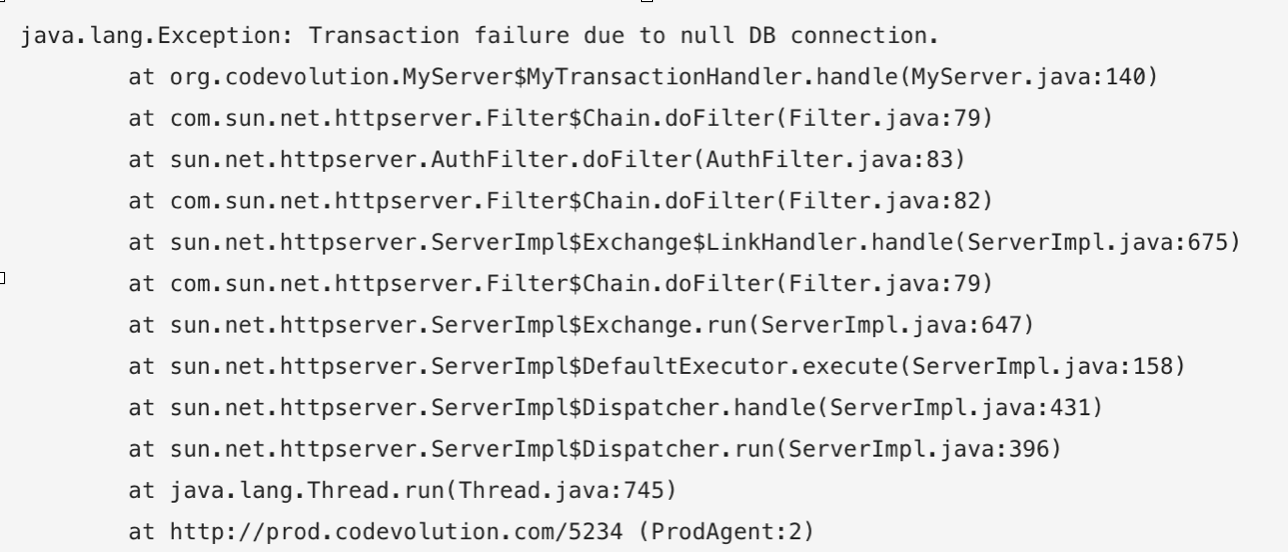
\includegraphics[width=\textwidth]{stack-with-link.png} 
    \begin{itemize}
  \item Are they locally defined?
  \item Are they static variables? 
  \item Are they arrays?
  \item Are they objects?
\end{itemize}


  \caption[Stack-trace with portal dashboard link]{Notice the link at the bottom of the stack.}
\end{figure}

This is currently achieved by adding an additional java.lang.StackTraceElement entry into the stack-trace. There are a few alternatives through which this can be implemented less intrusively, but this implementation was sufficient for all intents and purposes of this MVP, guaranteeing that any logging system which would record the stack-trace would also pick-up the URL to where it can be viewed in the Dashboard.

\subsubsection{Operating System specific code}
Compiler defined constants were used to customise the behaviour of the agent based on the operating system it is compiled for \cite{compiler}.

Two of the most important operating system specific parts were the threading library (windows.h vs pthread.h) and the JDK (win32 vs darwin).

\subsubsection{Building pipeline}
A few small scripts drive the building pipeline which quickly and predictably builds the Agent into libraries for different operating systems (.dylib, .dll and .so).

Moreover, the pipeline also takes care of building the test Java app used to assess the behaviour of the agent.


\subsection{API}
\subsubsection{Overview}
The API engine was built in Scala v2.11.8 using the Spray v1.3.3 Library for handling HTTP requests and the SBT tool for dependency management.

The ReactiveMongo v0.11.14 library provided the adaptor for communicating with the MongoDB database.

The codebase has been split into three main parts
\begin{itemize}
  \item Models, which are Scala objects and their writers and readers for conversion to JSON and to/from Mongo. Examples: User, UserApp, Log
  \item Providers, which interact with Mongo to obtain data. There generally is one provider for each Mongo collection used by the API. examples: UserProvider, LogProvider, AppProvider 
  \item Services, which define groups of request routes for different behaviours such the group handling authentication and the group handling app log submission and retrieval requests.
\end{itemize}


A quick look at the protocol used to communicate with the API from the point of view of the Agent and the Dashboard will be presented next.

\subsubsection{Agent app state messages}
There are three types of messages which represent the running state of an instance of an app.

The Start event can be accompanied by additional system properties data which could be used to differentiate between instances of the same app and provide additional debugging information in the Dashboard.

These messages are sent to the /log endpoint.

\begin{listing}[H]
\begin{minted}{xml}
    <app>
        <event>start</event>
        <hostname>My-MacBook-Pro.local</hostname>
        <pid>77764</pid>
        <command>./release/app.jar</command>
        <p_name>/usr/bin/java</p_name>
        <c_path>./release/app.jar</c_path>
        <jvm>Java HotSpot(TM) 64-Bit Server VM</jvm>
        <agentv>1.0.0</agentv>
    </app>
\end{minted}
\caption{XML start app message from agent to API}
\end{listing}



\begin{listing}[H]
\begin{minted}{xml}
    <app>
        <event>ping</event>
    </app>
\end{minted}
\caption{XML heartbeat message from agent to API}
\end{listing}



\begin{listing}[H]
\begin{minted}{xml}
    <app>
        <event>stop</event>
    </app>
\end{minted}
\caption{XML shutdown message from agent to API}
\end{listing}


\subsubsection{Agent log submit message}
This message contains the representation of an exception's details.

A few properties are recorded at the beginning, such as whether it has been caught or not, and if yes then by which method it is handled.  

A list of specifics for all the objects which were relevant to the stack trace follows (if they were found multiple times, they are recorded only once in this object list). Each entry contains the unique id, name, identified source, signature and value.

A final list, this time of stack-trace frames, completes the message. Each entry specifies the different variables the frame contains. If the variable was not an object, its value is specified right on the spot, otherwise it is cross-referenced to the object list.

These messages are sent to the /log endpoint.

\begin{listing}[H]
\begin{minted}{xml}
  <caught l="">
     <m><![CDATA[run]]></m>
     <sig><![CDATA[Lorg/codevolution/MyServer$1;]]></sig>
     <s><![CDATA[MyServer.java]]></s>
  </caught>
  <getMessage>
    <![CDATA[Manually thrown timer based custom exception]]>
  </getMessage>
  <objects>
     <v id="1447195560">
        <n>this</n>
        <s>Lorg/codevolution/MyServer$1;</s>
        <v><![CDATA[org.codevolution.MyServer$1@564273a8]]></v>
     </v>
  </objects>
  <sts>
     <st l="">
        <m><![CDATA[run]]></m>
        <sig><![CDATA[Lorg/codevolution/MyServer$1;]]></sig>
        <s><![CDATA[MyServer.java]]></s>
        <vars>
           <v>
              <n>testExceptionVar</n>
              <s>I</s>
              <v><![CDATA[5]]></v>
           </v>
           <v id="1447195560" />
        </vars>
     </st>
     <st l="">
        <m><![CDATA[mainLoop]]></m>
        <sig><![CDATA[Ljava/util/TimerThread;]]></sig>
        <s><![CDATA[Timer.java]]></s>
        <vars />
     </st>
     <st l="">
        <m><![CDATA[run]]></m>
        <sig><![CDATA[Ljava/util/TimerThread;]]></sig>
        <s><![CDATA[Timer.java]]></s>
        <vars />
     </st>
  </sts>
\end{minted}
\caption{XML stack-trace log message from agent to API}
\end{listing}




\subsubsection{Dashboard specific endpoints}

Multiple other endpoints exist such as those necessary for authentication, fetching user apps/stack-trace data, creating apps and registering accounts. It is beyond the scope of this report to go in-depth about them.

\subsection{Dashboard Portal}
\subsubsection{Overview}
Three main use cases were decided from the beginning drove the development of the dashboard:

\begin{itemize}
  \item User account - Account creation and session management
  \item Apps management - User apps view and app creation ability
  \item App management - Processed events list
  \item In-depth stack-trace - Log data exploration  
\end{itemize}

\subsubsection{Use case - User account}
\begin{figure}[H]
  \centering
    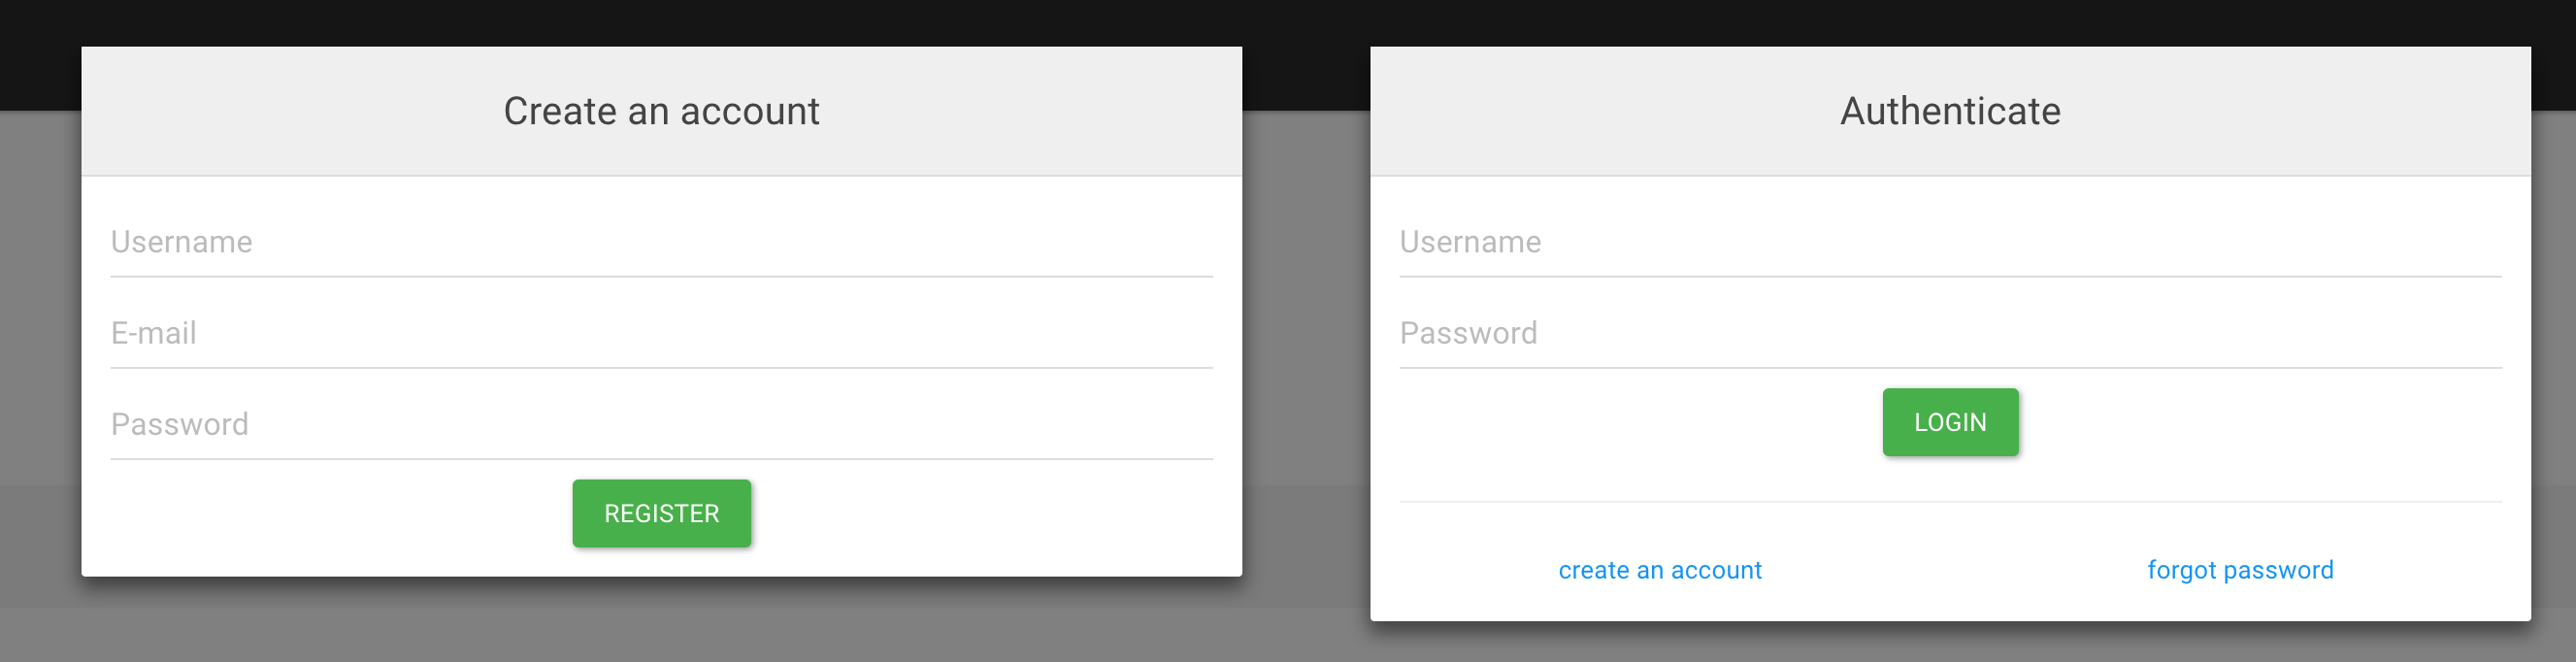
\includegraphics[width=\textwidth]{dashboard-account.png} 
  \caption[Dashboard - User account]{Dashboard - User account}
\end{figure}

The user can accomplish the task of authenticating on the Dashboard through the following
\begin{itemize}
  \item Quickly creating an account
  \item Using registration details to authenticate and explore data
\end{itemize}

\subsubsection{Use case - Apps management}
\begin{figure}[H]
  \centering
    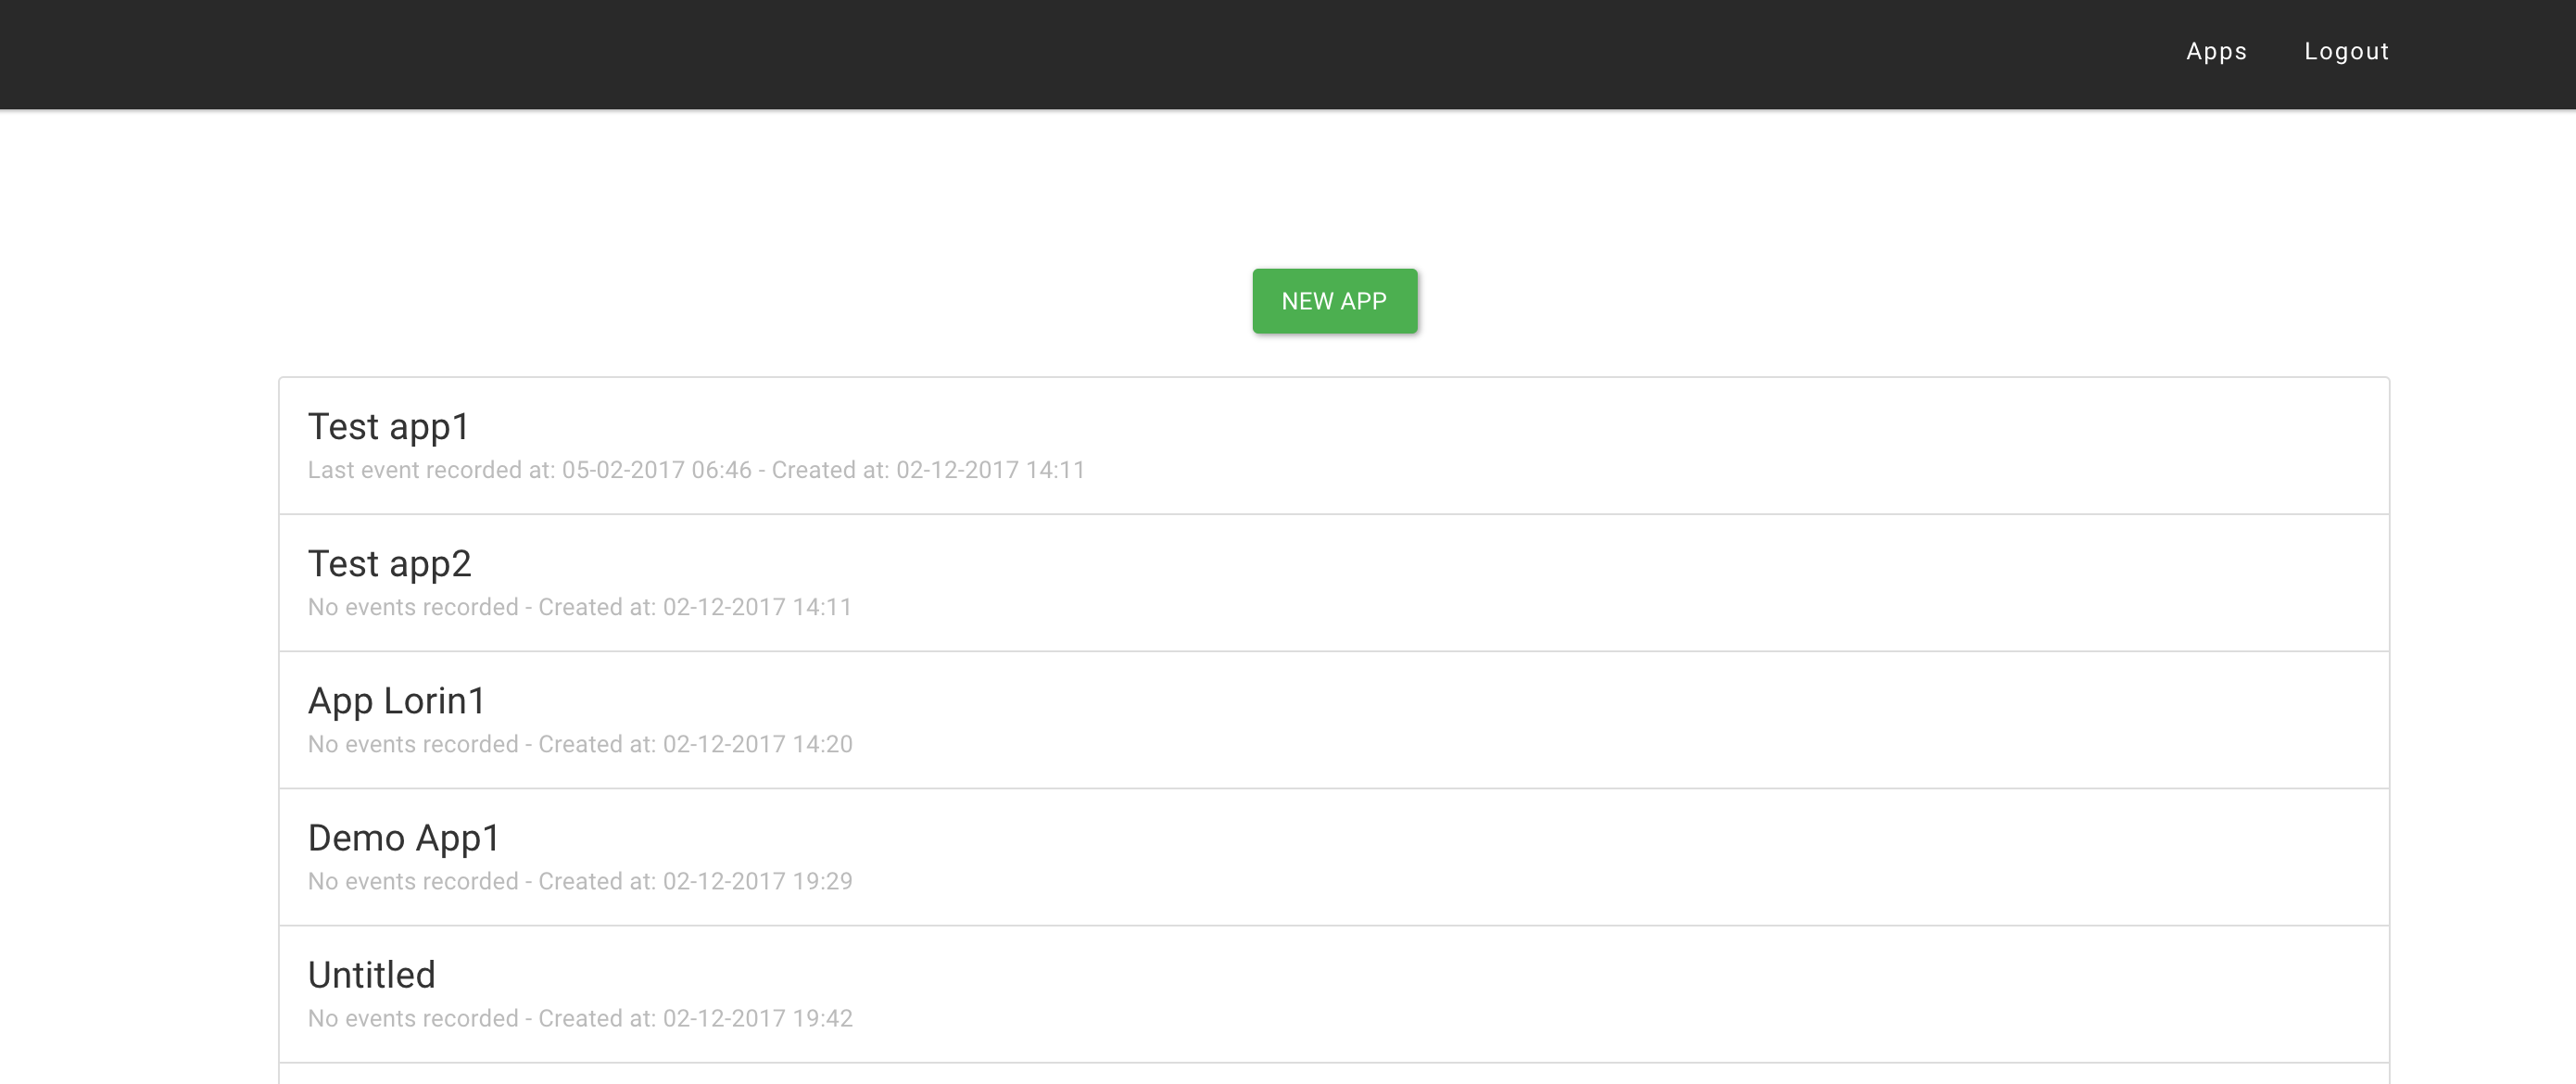
\includegraphics[width=\textwidth]{dashboard-apps.png} 
  \caption[Dashboard - Apps management]{Dashboard - Apps managements}
\end{figure}

The user can accomplish the task of managing his apps through the following
\begin{itemize}
    \item Creating a new app
  \item Viewing a list of created apps with the ability to move to a secondary in-depth view for each one
  \item Additional information provided for each app such as when the last even has come in
\end{itemize}

\subsubsection{Use case - User-app management}

\begin{figure}[H]
  \centering
    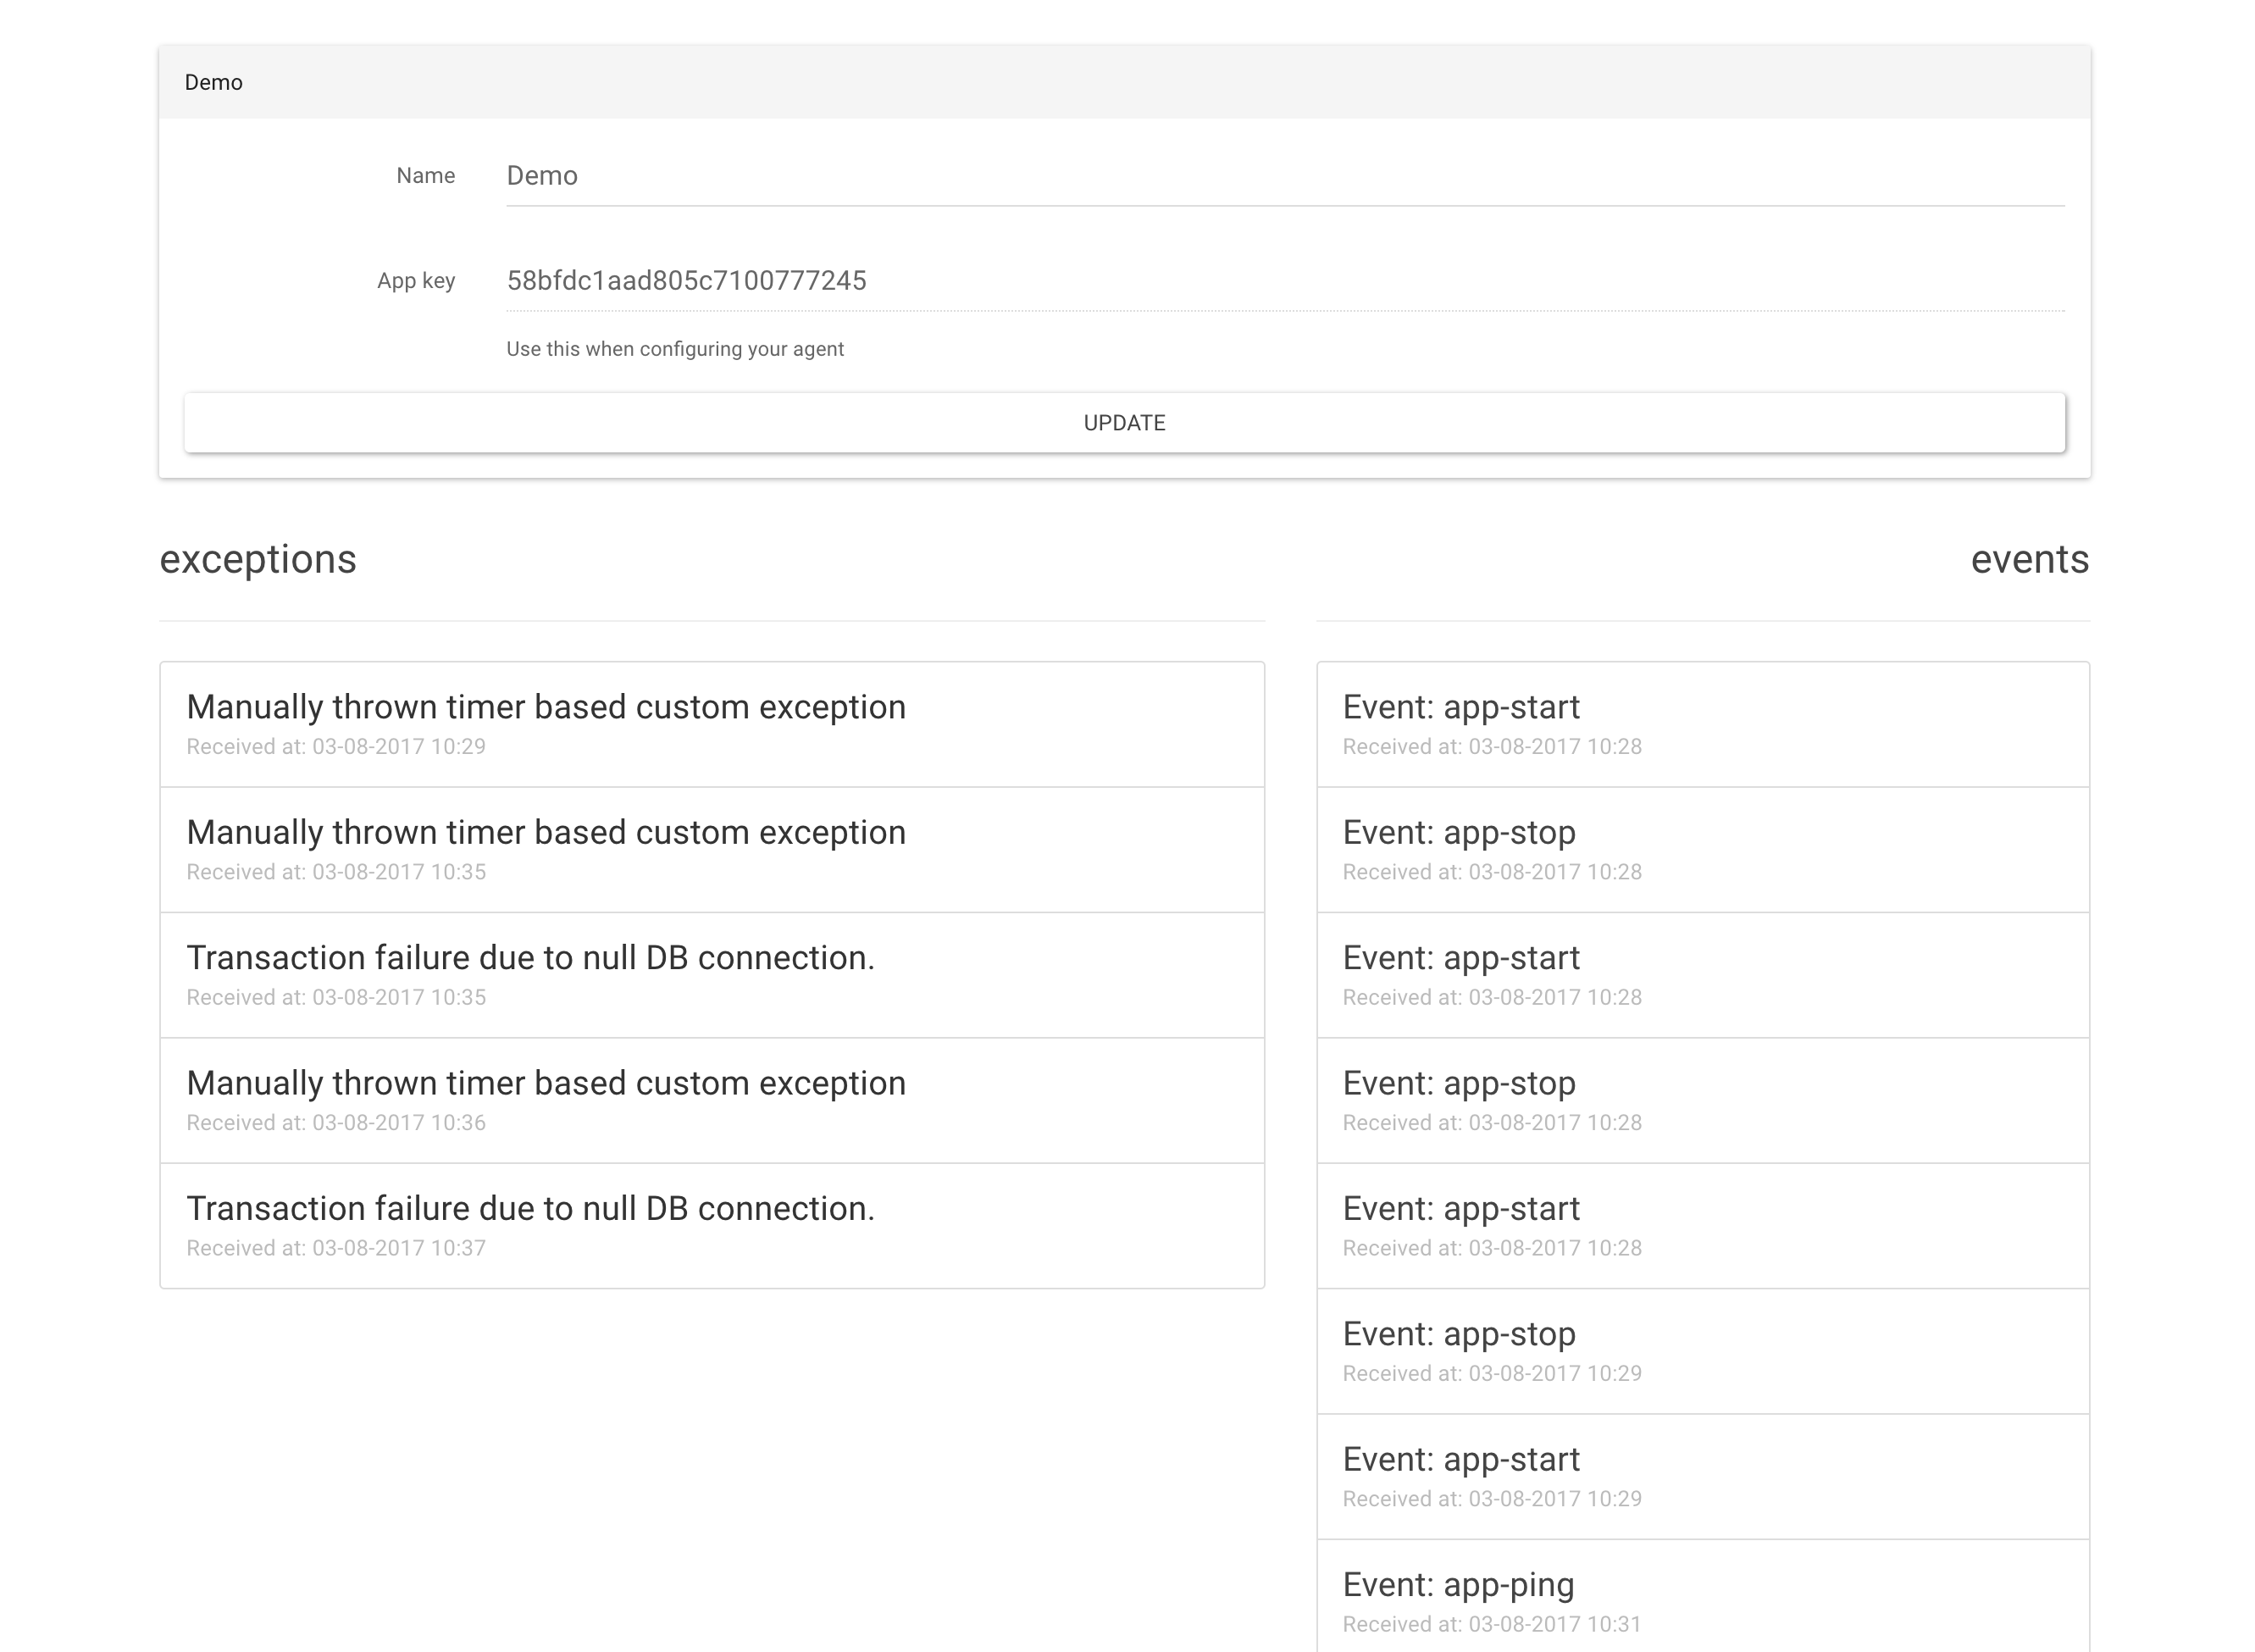
\includegraphics[width=\textwidth]{dashboard-app.png} 
  \caption[Dashboard - User-app management]{Dashboard - User-app management}
\end{figure}

The user can accomplish the task of managing his app through the following
\begin{itemize}
  \item Update basic details to customise the app configuration, such as its name
  \item Obtain the App key needed as an input to the Agent
  \item Explore recorded exceptions with the ability to move to a secondary in-depth view for each one
  \item View other events captured for the app such as the known start and shutdown times
\end{itemize}



\subsubsection{Use case - In-depth stack-trace view}

\begin{figure}[H]
  \centering
    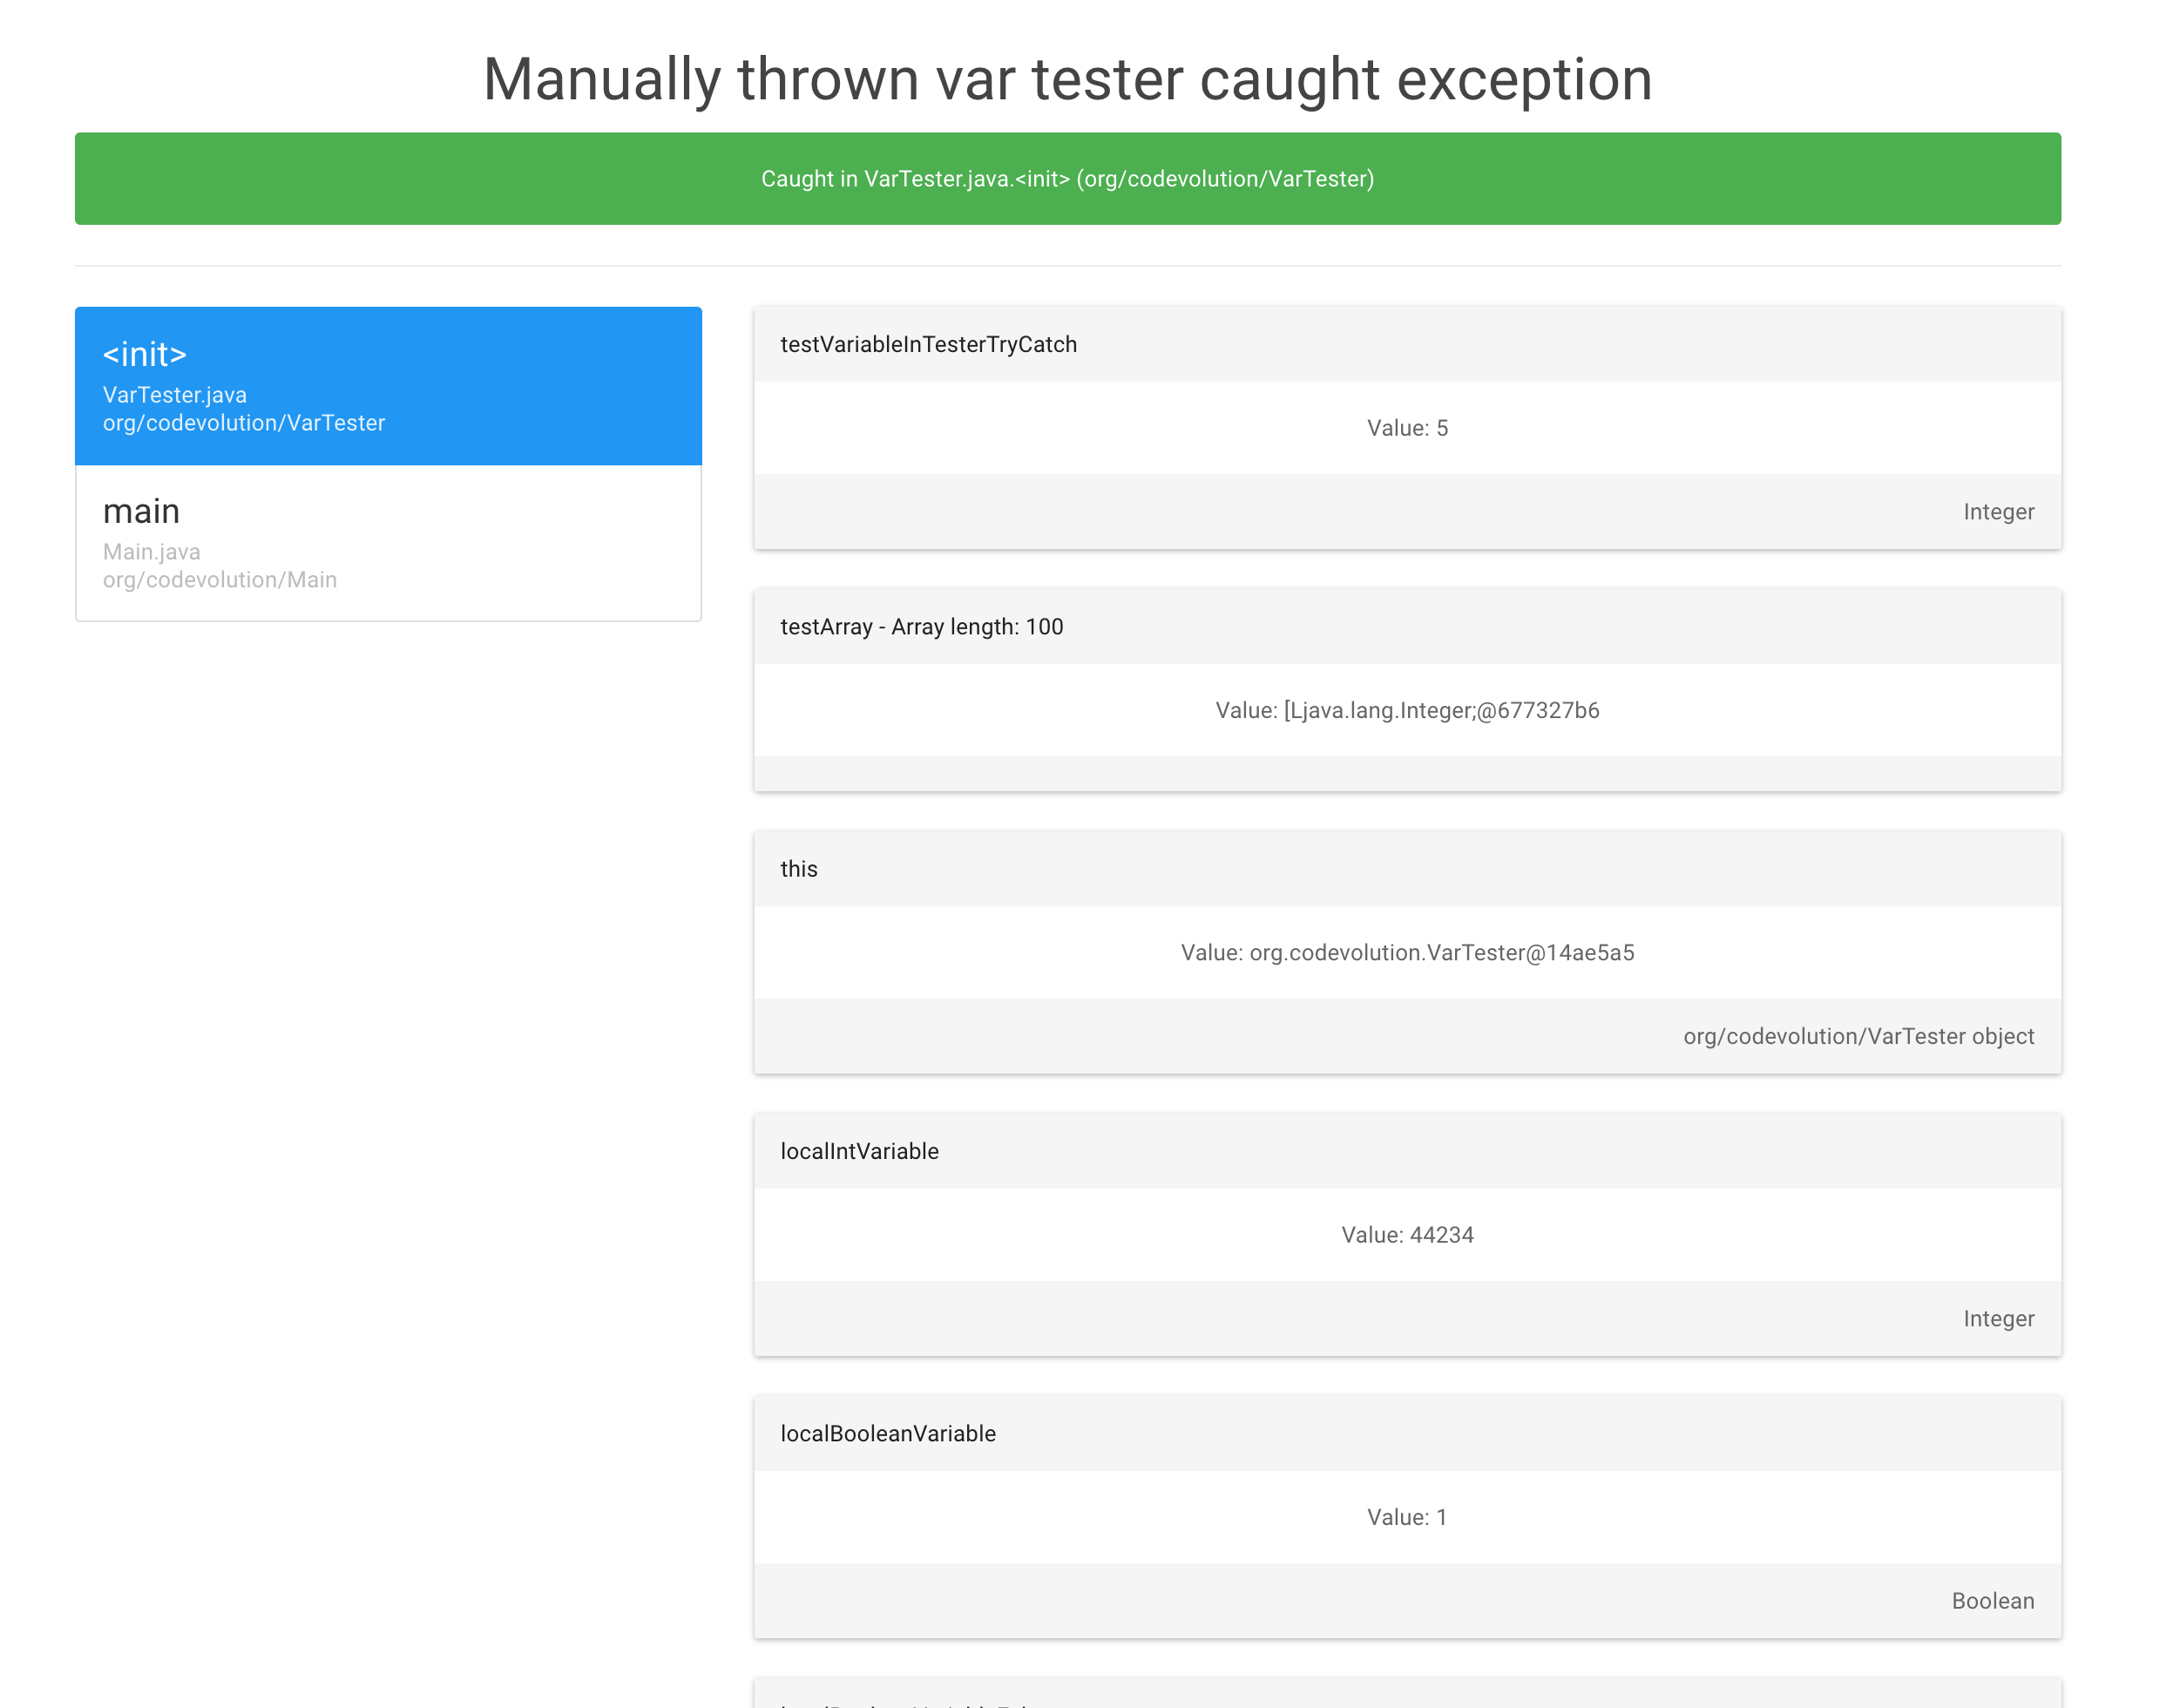
\includegraphics[width=\textwidth]{dashboard-exception.png} 
  \caption[Dashboard - In-depth stack-trace view]{Dashboard - In-depth stack-trace view}
\end{figure}

The XML stored for each stack-trace is parsed at this point in the controller of this view to then allow the view to match the variables inside the currently selected frame/method to the map of objects on a per-need basis. The format of the XML is explained in the Implementation section.

The user can accomplish the task of in-depth exploration of a recorded stack-trace through the following
\begin{itemize}
  \item Navigating from one frame of the stack-trace to another
  \item Visualising variables, with automatic mapping to human-readable types and values, per frame
  \item Availability of information on how the exception was handled app-side
\end{itemize}



\newpage